\lab{Policy Function Iteration}{Policy Function Iteration}
\objective{Iterative methods can be powerful ways to solve dynamic optimization problems without computing the exact solution.
Often we can iterate very quickly to the true solution, or at least within some $\epsilon$ error of the solution.
These methods are significantly faster than computing the exact solution using dynamic programming.
We demonstrate two iterative methods, value iteration and policy iteration, and we use them to solve a deterministic Markov decision process.}

\section*{Dynamic Optimization}

Many dynamic optimization problems take the form of a \emph{Markov decision process}.
A Markov decision process is similar to that of a Markov chain, but rather than determining state movement using only probabilities, state movement is determined based on probabilities, actions, and rewards.
They are formulated as follows.

$\mathbb{T}$ is a set of discrete time periods.
In this lab, $\mathbb{T} = {0,1,\ldots, L}$, where $L$ is the final time period.
$S$ is the set of possible states.
The set of allowable actions for each state $s$ is $A_s$.
$s_{t+1}=g(s_t,a_t)$ is a transition function that determines the state $s_{t+1}$ at time $t+1$ based on the previous state $s_t$ and action $a_t$.
The reward $u(s_t,a_t,s_{t+1})$ is the reward for taking action $a$ while in state $s$ at time $t$ and the next state being state $s_{t+1}$.

The time discount factor $\beta \in [0,1]$ determines how much the reward function decreases in value with time.
Looking at the cake eating problem described in the previous lab, the cake goes stale with each passing day.
In other words, each day you do not finish the cake, the reward of eating a piece decreases.
$\beta$ accounts for this decrease in value.

Let $N_{s,a}$ be the set of all possible next states when taking action $a$ in state $s$.
$p(s_t,a_t,s_{t+1})$ is the probability of taking action $a$ at time $t$ while in state $s$ and arriving at state $s_{t+1}\in N_{s,a}$.
A deterministic Markov process has $p(s_t,a_t,s_{t+1}) = 1$ $\forall s,a$.
This means that $N_{s,a}$ has one element $\forall s,a$.
A stochastic Markov process has $p(s_t,a_t,s_{t+1})\leq 1$, which implies that there can be multiple possible next states for taking a given action in a given state.
As a result, $N_{s,a}$ has multiple elements for each $s,a$.

The dynamic optimization problem is

\begin{align}
\label{eq:policyiter-dynopt1}
\max_\mathbf{a}  & \sum_{t=0}^{L} \beta^t u(s_t,a_t) \\
\mbox{subject to } & s_{t+1}= g(s_t,a_t)\ \forall t.
\end{align}

The cake eating problem follows this format where $S$ consists of the possible amounts of remaining cake ($\frac{i}{W}$), $c_t$ is the amount of cake we can eat, and the amount of cake remaining $s_{t+1}=g(s_t,a_t)$ is $w_t-c_t$, where $w_t$ is the amount of cake we have left and $c_t$ is the amount of cake we eat at time $t$.
This is an example of a deterministic Markov process.

For this lab, we define a dictionary $P$ to represent the decision process.
This dictionary contains all of the information about the states, actions, probabilities, and rewards.
Each dictionary key is a state-action combination and each dictionary value is a list of tuples.
\[P[s][a]=[(p(s,a,\bar{s}), \bar{s}, u(s,a,\bar{s}), is\_terminal),...]\]

Note the slight notation change from $(s_t,a_t,s_{t+1})$ to $(s,a,\bar{s})$. In the dictionary, $s$ is the current state, $a$ is the action, $\bar{s}\in N_{s,a}$ is the next state if action $a$ is taken, and \emph{is\_terminal} indicates if $\bar{s}$ is a stopping point.
In addition, $p(s,a,\bar{s}) $ is the probability of taking action $a$ while in state $s$, and $u(s,a,\bar{s})$ is the reward for taking action $a$ while in state $s$.

\subsection*{Moving on a Grid}

Now consider an $N \times N$ grid.
Assume that a robot moves around the grid, one space at a time, until it reaches the lower right hand corner and stops.
Each square is a state, $S = \{0, 1, \ldots, N^2-1\}$, and the set of actions is $\{Left, Down, Right, Up\}$.
For this lab, $Left = 0$, $Down = 1$, $Right = 2$, and $Up = 3$.
If you take the action $a = 1$, then you move \emph{Down} on the grid.

Let $N=2$ and label the squares as displayed below.
In this example, we define the reward to be -1 if the robot moves into state 2, -1 if the robot moves into state 0 from state 1, and 1 when it reaches the end state, state 3.
We define the reward function to be $u(s,a,\bar{s}) = u(\bar{s})$.
Since this is a deterministic model, $p(s,a,\bar{s}) = p(\bar{s}) = 1$ for all possible $s,a$.

\begin{center}
\begin{tabular}{|c|c|}
\hline
0 & 1 \\ \hline
\cellcolor{red!20}2 & \cellcolor{green!20}3 \\ \hline
\end{tabular}
\end{center}

$A_s$ is the set of actions that keep the robot on the grid.
If the robot is in the top left hand corner, the only allowed actions are $Down$ and $Right$ so $A_0 = \{1,2\}$.
The transition function $g(s,a) = \bar{s}$ can be explicitly defined for each $s, a$ where $\bar{s}$ is the new state after moving.

%\begin{align*}
%S &= \{0, 1, 2, 3\}\\
%A_0 &= \{Right, Down\} &A_1 &= \{Left, Up\} &A_2 &= \{Up, Right\} & A_3 &= \{\} \\
%g(0,Right) &= 1 &g(1,Left) &= 0 &g(2,Up) &= 0\\
%g(0,Down) &= 2 &g(1,Down) &= 3 &g(2,Right) &= 3 \\
%u(0) &= 0 &u(1) &= 0 &u(2) &= -1 &u(3) &= 1 \\
%p(0) &= .75 &p(1) &= .25 &p(2) &= .75 &p(3) &= .25
%\end{align*}

All of this information is encapsulated in $P$.
We define $P[s][a]$ for all states and actions, even if they are not possible.
This simplifies coding the algorithm but is not necessary.

\begin{center}
\begin{tabular}{llll}
\li{P[0][0] = [(0, 0, 0, False)]}
    & \li{P[2][0] = [(0, 2, -1, False)]}\\
\li{P[0][1] = [(1, 2, -1, False)]}
    & \li{P[2][1] = [(0, 2, -1, False)]}\\
\li{P[0][2] = [(1, 1, 0, False)]}
    & \li{P[2][2] = [(1, 3, 1, True)]}\\
\li{P[0][3] = [(0, 0, 0, False)]}
    & \li{P[2][3] = [(1, 0, 0, False)]}\\
\li{P[1][0] = [(1, 0, -1, False)]}
    &\li{P[3][0] = [(0, 0, 0, True)]} \\
\li{P[1][1] = [(1, 3, 1, True)]}
    &\li{P[3][1] = [(0, 0, 0, True)]}\\
\li{P[1][2] = [(0, 0, 0, False)]}
    &\li{P[3][2] = [(0, 0, 0, True)]}\\
\li{P[1][3] = [(0, 0, 0, False)]}
    &\li{P[3][3] = [(0, 0, 1, True)]}
\end{tabular}
\end{center}

For the sake of clarity, we will do a quick example using the above dictionary.
We first assume that we start in state 0 corresponding to the 0 in the above grid.
Next, we move $Down$ the grid to state 2.
This corresponds to taking action 1.
To get the correct values from the dictionary, we look at $P[s][a]$ or in this case $P[0][1] = [(1,2,-1,False)]$. 
So, when we move $Down$ from state 0 to state 2, $p(\bar{s}) = 1$,  $u(\bar{s}) = -1$, and $\bar{s} = 2$.
As a final note, when the action is not possible $p(\bar{s}) = 0$, as shown in the dictionary above.

We define the \emph{value function} $V(s)$ to be the maximum possible reward of starting in state $s$.
Then using Bellman's optimality equation,
\begin{equation}
\label{eq:policyiter-val-func}
V(s) = \max_{a \in A_s} \left\{\sum_{\bar{s}\in N_{s,a}}p(\bar{s}) * \left( u(\bar{s}) + \beta V(\bar{s})\right)\right\}.
\end{equation}

The summation occurs when it is a stochastic Markov process.
For example, if the robot is in the top left corner and we want it to move right, we could have the probability of the robot actually moving right as 0.5.
In this case, $P[0][2] = [(0.5, 1, 0, False), (0.5, 2, -1, False)]$.
This type of process will occur later in the lab.

\section*{Value Iteration}

In the previous lab, we used dynamic programming to solve for the value function.
This was a recursive method where we calculated all possible values for each state and time period.
\emph{Value iteration} is another algorithm that solves the value function by taking an initial value function and calculating a new value function iteratively.
Since we are not calculating all possible values, it is typically faster than dynamic programming.

\subsection*{Convergence of Value Iteration}

A function $f$ that is a contraction mapping has a \emph{fixed point} $p$ such that $f(p) = p$.
Blackwell's contraction theorem can be used to show that Bellman's equation is a ``fixed point'' (it actually acts more like a fixed function in this case)
for an operator $T: L^{\infty}(X;\mathbb{R}) \to L^{\infty}(X;\mathbb{R})$ where $L^{\infty}(X;\mathbb{R})$ is the set of all bounded functions:
\begin{equation}
\label{eq:policyiter-blackwell}
T[f](s) = \max_{a \in A_s} \left\{\sum_{\bar{s}\in N_{s,a}} p(\bar{s}) * \left( u(\bar{s}) + \beta f(\bar{s})\right)\right\}
\end{equation}
It can be shown that Equation \ref{eq:policyiter-dynopt1} is the fixed ``point'' of our operator $T$.
A result of contraction mappings is that there exists a unique solution to Equation \ref{eq:policyiter-blackwell}, namely

\begin{equation}
\label{eq:policyiter-val-iteration}
V_{k+1}(s_i) = T[V_k](s_i) = \max_{a \in A_s} \left\{\sum_{\bar{s}\in N_{s,a}}p(\bar{s}) *\left( u(\bar{s}) + \beta V_k(\bar{s})\right)\right\}
\end{equation}
where an initial guess for $V_0(s)$ is used.
As $k \to \infty$, it is guaranteed that $(V_k(s)) \to V^*(s)$.
Because of the contraction mapping, if $V_{k+1}(s) = V_k(s) \, \, \forall \, s$, we have found the true value function, $V^*(s)$.
% Using this information, we define the value iteration algorithm to find $V^*$:

% \begin{algorithm}[H]
% \begin{algorithmic}[1]
% \Procedure{Value Iteration Function}{$P, S, A, \beta, \varepsilon$, maxiter}
%     \State $V_0 \gets [V_0(s_0),V_0(s_1),\ldots,V_0(s_N)] $
%      \Comment{Common choice is $V_0(s_i)=u(s_i)$}
%     \For{$i=1,2,\dots,$\ \li{maxiter}}
%         \Comment Iterate only \li{maxiter} times at most.
%         \For{$s \in S$}
%              \State $V_{k+1}(s) = \max_{a \in A_s}\{\Sigmap(a)*(u(a) + \beta*V_k(a))]\}$
%         \EndFor
%         \If{ $||V_{k+1} - V_k|| < \varepsilon$}
%             \State \texttt{break}
%              \Comment{Stop iterating if the approximation stops changing enough.}
%         \EndIf
%     \EndFor
%     \State \pseudoli{return} $V_k$
% \EndProcedure
% \end{algorithmic}
% \caption{Value Function Iteration}
% \label{alg:ValueIteration}
% \end{algorithm}

As an example, let $V_0 = [0,0,0,0]$ and $\beta = 1$, where each entry of $V_0$ represents the maximum value at that state, and $V_0(s) = V_0[s]$ if we are using the array or list form of the \emph{value function}.
We calculate $V_1(s)$ from the robot example above.
For $V_1(0)$, we choose the \li{max} of the possible outcomes, states 1 or 2, after moving.
Thus we use $P[0][2]$ for state 1 because moving from state 0 to state 1 requires going right, action 2.

\begin{align*}
V_1(0) &= \max_{a \in A_0} \left\{\sum_{\bar{s}\in N_{s,a}}p(\bar{s})*(u(\bar{s})+V_0(\bar{s}))\right\} \\
&= \max \{p(1)*(u(1)+V_0(1)), p(2)*(u(2)+V_0(2)))\} \\
&= \max \{1(0+0), 1(-1+0)\} \\
&= \max \{0,-1\} \\
&= 0 \\
V_1(1) &= \max \{p(0)*(u(0)+V_0(0)), p(3)*(u(3)+V_0(3))\} \\
&=\max \{1(-1+0), 1(1+0)\} \\
&= 1 \\
V_1(2) &= \max\{p(0)*(u(0)+V_0(0)), p(3)*(u(3)+V_0(3))\} \\
&=\max \{1(0+0),1(1+0)\} \\
&= 1 \\
V_1(3) &= \max\{p(1)*(u(1)+V_0(1)), p(2)*(u(2)+V_0(2))\} \\
&=\max \{1(0+0),1(0+0)\} \\
&= 0
\end{align*}
This calculation gives $V_1 = [0, 1, 1, 0]$.
Repeating the process yields $V_2 = [1, 1, 1, 0]$. Repeating a third time gives $V_3 = [1, 1, 1, 0]$, which is the same as $V_2$, so the process has converged. This means that the solution is $[1, 1, 1, 0]$.
Thus, the total maximum reward the robot can achieve by starting on square $i$ is the $i$th entry of the solution $[1, 1, 1, 0]$.

When implementing functions in this lab, instead of only looking at possible actions $a\in A_s$, we can consider all of the actions.
This will not affect the results, because $p(\bar{s}) = 0$ when an action is not possible.
This simplifies the coding significantly.
For example, when calculating $V_{k+1}(s_i)$ consider the following lines of code.

\begin{lstlisting}
sa_vector = np.zeros(nA)
for a in range(nA):
    for tuple_info in P[s][a]:
        # tuple_info is a tuple of (probability, next state, reward, done)
        p, s_, u, _ = tuple_info
        # sums up the possible end states and rewards with given action
        sa_vector[a] += (p * (u + beta * V_old[s_]))
#add the max value to the value function
V_new[s] = np.max(sa_vector)
\end{lstlisting}

% Most iterative algorithms have a \li{maxiter} parameter that will terminate the algorithm after \li{maxiter} iterations regardless of whether or not it has converged.
% This is because even though we have guaranteed convergence, we might have a convergence rate that is too slow to be useful.
% However, generally this algorithm will converge much faster than computing the true value function using dynamic programming.

\begin{problem}
\label{prob:policyiter-value1}
Write a function called \li{value_iteration()} that will accept a dictionary $P$ representing the decision process, the number of states, the number of actions, a discount factor $\beta \in (0,1]$ defaulting to 1, the tolerance amount $\epsilon$ defaulting to \li{1e-8}, and the maximum number of iterations \li{maxiter} defaulting to 3,000.
Perform value iteration until $\|V_{k+1} - V_{k}\| < \epsilon$ or $k > $ \li{maxiter}.
Return the final vector representing $V^*$ and the number of iterations.
Test your code on the example given above.
\end{problem}

\subsection*{Calculating the Policy}

While knowing the maximum expected value is helpful, it is usually more important to know the policy that generates the most value.
Value iteration tells the robot what reward it can expect, but not how to get it.
The policy vector is found by using the policy function: $\pi : \mathbb{R} \to \mathbb{R}$.
$\pi(s)$ is the action that should be taken while in state $s$ to maximize the reward.
We can modify the Bellman equation using $V^*(s)$, which is the true value function we found in Problem \ref{prob:policyiter-value1}, to find $\pi$:
\begin{equation}
\label{eq:policyiter-pol_func}
\pi(s) = \argmax_{a \in A_s} \left\{\sum_{\bar{s}\in N_{s,a}} p(\bar{s})*(u(\bar{s}) + \beta*V^*(\bar{s}))\right\}
\end{equation}

Using value iteration, we found $V^*  = [1, 1, 1, 0]$ in the example above.
We find $\pi(0)$ from the example above with $\beta = 1$ by looking at actions $1$ and $2$ (since actions 0 and 3 have probability 0).
\begin{align*}
\pi(0) &=\argmax_{1,2} \{p(2)*(u(2) + V^*(2)), p(1)*(u(1)+V^*(1))\} \\
&= \argmax \{1*(-1+1), 1*(0+1)\} \\
&= \argmax\{0, 1\}\\
&= 2
\end{align*}

So when the robot is in state 0, it should take action 2, moving $Right$.
This avoids the -1 penalty for moving $Down$ into state 2.
Similarly,
\begin{align*}
\pi(1) &= \argmax_{0,1} \{1*(-1+1), 1*(1+0)\} \\
&= \argmax \{0, 1\} = 1 \\
\pi(2) &= \argmax_{2,3} \{1*(1+0), 1*(0+1)\} \\
&= \argmax \{1, 1\} = 2
\end{align*}
Since state 3 is terminal, it doesn't matter what $\pi(3)$ is, but we'll set it to 0 for convenience.
Thus, the policy corresponding to the optimal reward is $[2,1,2,0]$.
The robot should move to state 3 if possible, avoiding state 2 because it has a negative reward.

\begin{info}
Note that $\pi$ gives the optimal action $a$ to take at each state $s$.
It does not give a sequence of actions to take in order to maximize the policy.
\end{info}

\begin{problem}
\label{prob:policyiter-value2}
Write a function called \li{extract_policy()} that will accept a dictionary $P$ representing the decision process, the number of states, the number of actions, an array representing the value function, and a discount factor $\beta \in (0,1]$ defaulting as before.
Return the policy vector corresponding to $V^*$.
Test your code on the example with $\beta = 1$.
\end{problem}

\section*{Policy Iteration}
For dynamic programming problems, it can be shown that value function iteration converges relative to the discount factor $\beta$.
As $\beta\rightarrow1$, the number of iterations increases dramatically.
As mentioned earlier $\beta$ is usually close to 1, which means this algorithm can converge slowly.
In value iteration, we used an initial guess for the value function, $V_0$ and used Equation \ref{eq:policyiter-dynopt1} to iterate towards the true value function.
Once we achieved a good enough approximation for $V^*$, we recovered the true policy function $\pi^*$.
Instead of iterating on our value function, we can instead make an initial guess for the policy function, $\pi_0$, and use this to iterate toward the true policy function.
We do so by taking advantage of the definition of the value function, where we assume that our policy function yields the most optimal result.
This is called \emph{policy iteration}.

That is, given a specific policy function $\pi_k$, we can modify Equation \ref{eq:policyiter-dynopt1} by assuming that the policy function is the optimal choice.
This process, called \emph{policy evaluation}, evaluates the value function for a given policy.

\begin{equation}
\label{eq:policyiter-val_from_policy}
V_{k+1}(s) = \max_{a \in [A_s]} \left\{\sum_{\bar{s}\in N_{s,a}} p(\bar{s})*(u(\bar{s}) + \beta *V_{k}(\bar{s}))\right\} =  \sum_{\bar{s}\in N_{s,\pi(s)}} p(\bar{s})*(u(\bar{s}) + \beta *V_{k}(\bar{s}))
\end{equation}
The last equality occurs because in state $s$, the robot should choose the action that maximizes the reward, which is $\pi(s)$ by definition.
Like value iteration, policy iteration iterates until the desired tolerance is reached.
This ensures that we get the value function that optimizes the reward for each starting state.

\begin{problem}
\label{prob:policyiter-value3}
Write a function called \li{compute_policy_v()} that accepts a dictionary $P$ representing the decision process, the number of states, the number of actions, an array representing a policy, a discount factor $\beta \in (0,1]$, and a tolerance amount $\epsilon$, defaulting as before.
Use the policy evaluation process above to return the value function corresponding to the policy.

Test your code on the policy vector generated from \li{extract_policy()} for the example.
The result should be the same value function array from \li{value_iteration()}.
\end{problem}

Now that we have the value function for our policy, we can take the value function and find a better policy.
This is called \emph{policy improvement}.
This step is the same method used in value iteration to find the policy.
In other words, this step uses the \li{extract_policy()} method from Problem \ref{prob:policyiter-value2} with the newly computed value function.

\emph{Policy function iteration} starts with an intial $\pi_{0}$ and iterates using policy evalutaion and policy improvement successively until the desired tolerance is reached.
The algorithm for policy function iteration, using two of the functions that you previously implemented, can be summarized as follows:

\begin{algorithm}[H]
\begin{algorithmic}[1]
\Procedure{Policy Iteration Function}{$P, nS, nA, \beta, tol,$ maxiter}
    \State $\pi_0 \gets [\pi_0(s_0),\pi_0(s_1),\ldots,\pi_0(s_N)] $
     %\Comment{Common choice is $\pi_0(w_i)=w_{i-1}$ with $\pi_0(0)=0$}
     \Comment{Initialize $\pi$ as array of ones of length \li{nS}}
    \For{$k=0,1,\dots,$\ \li{maxiter}}
        \Comment Iterate only \li{maxiter} times at most
        \State $V_{k+1}$ = compute\_policy\_v($\pi_{k}$)
        \Comment{Policy evaluation using \li{compute_policy_v()}}
        \State $\pi_{k+1}$ = extract\_policy($V_{k+1}$)
        \Comment{Policy improvement using \li{extract_policy()}}
        \If{ $||\pi_{k+1} - \pi_k|| < \varepsilon$}
            \State \texttt{break}
             \Comment{Stop iterating if the policy doesn't change enough}
        \EndIf
    \EndFor
    \State \pseudoli{return} $V_{k+1}, \pi_{k+1}$
\EndProcedure
\end{algorithmic}
\caption{Policy Iteration}
\label{alg:PolicyIteration}
\end{algorithm}

\begin{problem}
\label{prob:policyiter-value4}
Write a function called \li{policy_iteration()} that will accept a dictionary $P$ representing the decision process, the number of states, the number of actions, a discount factor $\beta \in (0,1]$, the tolerance amount $\epsilon$, defaulting as before, and the maximum number of iterations \li{maxiter} defaulting to 200.
Perform policy iteration until $\|\pi_{k+1} - \pi_{k}\| < \epsilon$ or $k > $ \li{maxiter}.
Return the final vector representing $V_k$, the optimal policy $\pi_k$, and the number of iterations.
Test your code on the example given above and compare your answers to the results from Problems \ref{prob:policyiter-value1} and \ref{prob:policyiter-value2}.
\\(Hint: This is just the \li{Policy Iteration} algorithm, except you also return the number of iterations)
\end{problem}

\section*{The Frozen Lake Problem}
For the rest of this lab, we will be using the Gymnasium environment \li{'FrozenLake-v1'}.
Gymnasium can be installed using the following code.
\begin{lstlisting}
>>> pip install gymnasium 
>>> # You may also need to install these dependencies
>>> pip install gymnasium[all]
>>> pip install gymnasium[classic-control]
\end{lstlisting}

In the Frozen Lake problem, an elf attempts to cross a treacherous frozen lake to obtain a present.
The lake is divided into an $N \times N$ grid where the top left corner is the start, the bottom right corner is the end, and the other squares are either frozen or holes.
To retrieve the present, the elf must successfully navigate around the melted ice without falling through.
The possible actions are left, right, up, and down, but since the ice is slippery, the elf won't always move in the intended direction.
Hence, this is a stochastic Markov process, i.e. $p(s_t,a_t,s_{t+1})<1$.
The reward for falling is 0, and the reward for obtaining the present is 1.
There are two scenarios with $N=4$ and $N=8$.

\begin{figure}
    \centering
    \begin{tabular}{cc}
        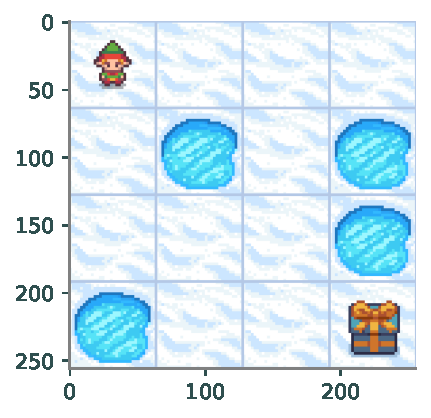
\includegraphics[width=.45\textwidth]{figures/4x4_image.pdf} &
        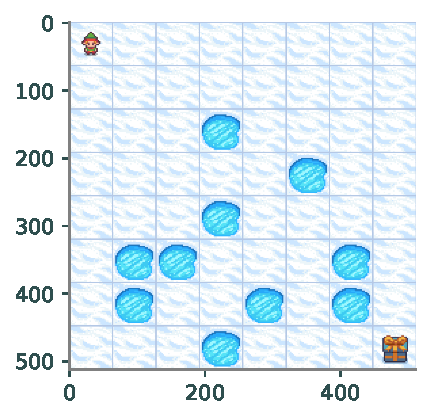
\includegraphics[width=.45\textwidth]{figures/8x8_image.pdf}
    \end{tabular}
    \caption{Default starting positions of the $4\times4$ and $8\times8$ versions of \li{"FrozenLake-v1"}}
    \label{fig:frozen_lake}
\end{figure}

\subsection*{Using Gymnasium}
The \li{'FrozenLake-v1'} environment has 3 important attributes, \li{P}, \li{obersavtion_space.n}, and \\ \li{action_space.n}.
We can calculate the optimal policy of \li{'FrozenLake-v1'} with value iteration or policy iteration using these 3 attributes.
Since the ice is slippery, this policy will not always result in a reward of 1.

\begin{lstlisting}
>>> import gymnasium as gym

>>> # Initialize environment for 4x4 scenario
>>> env = gym.make('FrozenLake-v1',desc=None,map_name='4x4',is_slippery=True)
>>> # Find number of states and actions
>>> env.obersavtion_space.n
16
>>> env.action_space.n
4
>>> # Get the dictionary with all the states and actions
>>> dictionary_P = env.P

>>> env.close()  # Always close the environment!
\end{lstlisting}

The attribute \li{P} is similar to the dictionary we used in the previous problems.
As already mentioned, $p(s_t,a_t,s_{t+1}) < 1$, which means the set $N_{s,a}$ has more than one value.
If you did not implement the functions in this lab to account for this, they will not work as intended on this dictionary, which we will use for the remainder of this lab.

\begin{problem}
\label{prob:policyiter-value5}
Write a function \li{frozen_lake()} that runs \li{value_iteration()}, \li{extract_policy()}, and \li{policy_iteration()} on FrozenLake.
It should accept a boolean \li{basic_case} defaulting to \li{True}, an integer $M$ defaulting to 1000 that indicates how many times to run the simulation, and a boolean \li{render} defaulting to \li{False}.
If \li{basic_case} is \li{True}, run the $4\times4$ scenario.
If not, run the $8\times8$ scenario.
If \li{render} is \li{True}, render the environment by applying the argument \li{render_mode='human'} when initializing the environment.
Close the environment at the end of the function.
(Hint: Rendering this environment can take a long time, so only render it with small values of $M$.)

Calculate and return the policy generated by value iteration, the mean total rewards of value iteration (set to 0 for now), the policy iteration value function, the policy generated by policy iteration, and the mean total rewards of policy iteration (also set to 0 for now).
\end{problem}

Gymnasium environments have built-in functions that allow us to simulate each step of the scenario.
Before running a simulation in Gymnasium, always revert it to the starting position by calling the \li{reset()} function.
The function \li{step()} moves the simulation to the next state.

\begin{lstlisting}
>>> import gymnasium as gym
>>> # Initialize environment for 4x4 scenario
>>> env = gym.make('FrozenLake-v1',desc=None,map_name='4x4',is_slippery=True)

>>> # Put environment in starting state
>>> observation, info = env.reset()
>>> # Take a step in the optimal direction and update variables
>>> observation, reward, done, trunc, info = env.step(int(policy[observation]))

>>> env.close()  # Always close the environment!
\end{lstlisting}

The function \li{step()} takes integers representing different actions and returns: \li{observation}, \li{reward}, \li{done}, \li{truncated}, and \li{info}.
When we take an action, we get a new \li{observation}, or state, as well as the \li{reward} for taking that action.
If the elf falls into a hole or reaches the present, the simulation terminates (\li{done=True}).
The \li{truncated} and \li{info} values will not be used in this lab.
For more information about this environment, visit \url{gymnasium.farama.org/environments/toy_text/frozen_lake/}.

\begin{problem}
\label{prob:policyiter-value6}
Write a function \li{run_simulation()} that takes in an environment \li{env}, a policy \li{policy}, and a discount factor $\beta$.
Calculate the total reward of the policy for one simulation of the environment (step through the environment until \li{done=True}).
This function will be called by \li{frozen_lake()}, which both initializes and closes the environment, so do not call \li{close()} in this function.
However, you should call \li{reset()} at the beginning of this function, to revert the environment back to its starting position.
\\(Hint: When calculating the reward, use $\beta^k$ as shown in Equation \ref{eq:policyiter-dynopt1}.)

Next, modify \li{frozen_lake()} to call \li{run_simulation()} for both the value iteration policy and the policy iteration policy $M$ times.
Then, modify \li{frozen_lake()} to return the actual values of the mean total reward for both policies.
\\(Hint: Even though you run the simulation $M$ times, you should only calculate the policies once, because each policy depends on the dictionary $P$, which does not change.)
\end{problem}


\begin{comment}
\newpage
%
%
%%\begin{equation}
%%\label{eq:policyiter-bellman1}
%%V(w_i) = \max_{c \in [0,w_i]} u(c) + \beta V(w_i-c)
%%\end{equation}
%%It is common to make the substitution $w_i' = w_i - c$ in \eqref{eq:policyiter-bellman1} to obtain the %following.
%\begin{equation}
%\label{eq:policyiter-bellman2}
%V(w_i) = \max_{w_j \in [0,w_i]} u(w_i-w_j) + \beta V(w_j).
%\end{equation}
%
%Notice that \eqref{eq:policyiter-bellman2} is similar to the value function given in the dynamic programming lab.
%%Note that \eqref{eq:policyiter-bellman1} requires finding $c$, how much cake to consume in each period.
%%The variable $c$ is commonly described as the \emph{action} to take when we have $w_i$ cake.
%
%
%\subsection*{Convergence of Value Iteration}
%
%A function $f$ that is a contraction mapping has a fixed point $p$ such that $f(p) = p$.
%Blackwell's contraction theorem can be used to show that Bellman's equation is a ``fixed point'' (it actually acts more like a fixed function in this case)
%for an operator $T: L^{\infty}(X;\mathbb{R}) \to L^{\infty}(X;\mathbb{R})$ where $L^{\infty}(X;\mathbb{R})$ is the set of all bounded functions:
%\begin{equation}
%\label{eq:policyiter-blackwell}
%[T(f)](w) = \max_{w_j \in [0,w]} u(w-w_j) + \beta f(w_j).
%\end{equation}
%It can be shown that (\ref{eq:policyiter-bellman2}) is the "fixed point" of our operator $T$.
%A result of contraction mappings is that there exists a unique solution to (\ref{eq:policyiter-blackwell}).
%
%A powerful property of contraction mappings is that the fixed point can be found by applying the function repeatedly to some initial point in our domain.
%That is, if $f:X \to X$ is our contraction mapping, with fixed point $p \in X$, we can find $p$ by randomly choosing $x \in X$ and repeatedly applying the function $f$ to our point.
%This can be expressed as
%\begin{align*}
%f^{M}(x) = f \circ f \cdots \circ f(x) = p
%\end{align*}
%for some M.  Here M is dependent on both the initial guess $x$ and the discount factor of the contraction mapping, which correspond to $V_0$ and $\beta$ in dynamic optimization.
%
%In the case of dynamic optimization, this implies that we can converge to the true value function $V^*(w)$ by using the following equation:
%\begin{equation}
%\label{eq:policyiter-val_iteration}
%V_{k+1}(w_i) = [T(V_k)](w_i) = \max_{w_j \in [0,w_i]} u(w_i-w_j) + \beta V_k(w_j) \, \, \forall \, w_i,
%\end{equation}
%
%where an initial guess for $V_0(w)$ is used.
%As $k \to \infty$, it is guaranteed that $(V_k(w)) \to V^*(w)$.
%Because of the contraction mapping, if $V_{k+1}(w) = V_k(w) \, \, \forall \, w$, we have found the true value function, $V^*(w)$.
%Using this information, we define the value iteration algorithm to find $V^*$:
%
%
%
%
%\begin{algorithm}[H]
%\begin{algorithmic}[1]
%\Procedure{Value Iteration Function}{$\beta, N, W, u(x), \varepsilon$, maxiter}
%    \State $w \gets [0, \frac{W}{N},\ldots, W]$
%      \Comment{Divide $W$ into $N$ equally sized pieces}
%    \State $V_0 \gets [V_0(w_0),V_0(w_1),\ldots,V_0(w_N)] $
%     \Comment{Common choice is $V_0(w_i)=u(w_i)$}
%    \For{$i=1,2,\dots,$\ \li{maxiter}}
%        \Comment Iterate only \li{maxiter} times at most.
%        \For{$w_i \in w$}
%            \State $V_{k+1}(w_i) = \max_{w_j \in \mathbf{w} \, | \, w_j \leq w_i} u(w_i-w_j) + \beta V_k(w_j)$
%        \EndFor
%        \If{ $||V_{k+1} - V_k|| < \varepsilon$}
%            \State \texttt{break}
%             \Comment{Stop iterating if the approximation stops changing enough.}
%        \EndIf
%    \EndFor
%    \State \pseudoli{return} $V_k$
%\EndProcedure
%\end{algorithmic}
%\caption{Value Function Iteration}
%\label{alg:ValueIteration}
%\end{algorithm}
%
%Most iterative algorithms have a \li{max\_iter} parameter that will terminate the algorithm after \li{max\_iter} iterations regardless of whether or not it has converged.
%This is because even though we have guaranteed convergence, we might have a convergence rate that is too slow to be useful.
%However, generally this algorithm will converge much faster than computing the true value function using dynamic programming as in Finite Value Iteration.
%
%\begin{warn} % Notation warning
%Note that $w_j \leq w_i$, because we can never have more cake at a later period; cake can only be consumed, not created.
%\end{warn}
%
%\begin{problem}
%\label{prob:policyiter-value1}
%Write a function called \li{value_iteration()} that will accept a numpy array representing the initial vector $V_0$, a discount factor $\beta \in (0,1)$,
%the number of states to split $\mathbf{w}$ into $N$, the amount of initial cake $W$, a utility function $u(x)$,
%the tolerance amount $\epsilon$, and the maximum number of iterations \li{max\_iter}.
%Perform value iteration until $\|V_{k+1} - V_{k}\| < \epsilon$ or $k > $ \li{max\_iter}.
%Return the final vector representing $V^*$.
%
%It is useful for our function to accept $V_0$ as a parameter instead of calculating an initial guess inside our function, so that we can try different initial states for $V_0$.
%
%Test your function with the parameters $N=400$, $\beta=.995$, $u(x)=\sqrt{x}$, $W=1$.
%Try different values for $V_0$ and see if you get the same value for $V^*(W)$ (The value should be approximately 9.4988).
%% Question to consider:
%How do different initial guesses for $V_0$ affect the number of iterations required for convergence?
%\end{problem}
%
%
%\subsection*{Policy Vector}
%
%The value function $V^*(w_i)$ that we found describes how much utility $w_i$ will yield over time, thus $V^*(W)$ is the optimal value for our problem:
%\begin{align*}
%  V^*(W) = \max_{c_t}  & \sum_{t=0}^T \beta^t u(c_t), \\
%  \mbox{subject to } & \sum_{t=0}^T c_t = W ,\\
%  & c_t \geq 0.
%\end{align*}
%Although $V^*(W)$ is the solution, it is usually more important to know which sequence of $(c_t)_{t=0}^T$ yields the solution.
%This sequence is known as the \emph{policy vector} $\mathbf{c} = [c_0, c_1, \ldots, c_T]$ that corresponds to eating $c_i$ cake at time $t=i$.
%
%If this were a truly infinite problem, $\mathbf{c}$ would be impossible to calculate; there would be an infinite number of time periods.
%Fortunately, in the cake-eating problem, we will never have more than $N$ time periods.
%This happens because it is never optimal to eat $0$ pieces of cake in a single time period.
%The discount factor $\beta$ means at least $1$ piece must be eaten at each step.
%It is important to note that the length of $\mathbf{c}$ changes depending on what $\beta$ is.
%When $\beta = 0$, for example, only the first time period matters because all the rest will yield zero utility.
%So when $\beta = 0$, $T = 0$ and the length of $\mathbf{c}$ is $1$.
%As the value of $\beta$ gets closer to $1$, $T$ increases as well.
%
%The policy vector, $\mathbf{c}$, is found by using the policy function: $\pi : \mathbb{R} \to \mathbb{R}$ which has the constraint $0 \leq \pi(w_i) \leq w_i \, \, \forall \, i.$
%$\pi(w_i)$ is the amount of cake to save for the next period, given we started with $w_i$ cake.
%In \eqref{eq:policyiter-val_iteration}, this was represented by $w_j$.
%
%Because $\pi(w_i)$ is the amount of cake saved until next period, we can use $V^*(W)$ and modify the Bellman equation to find $\pi$:
%\begin{equation}
%\label{eq:policyiter-pol_func}
%\pi(w_i) = \argmax_{w_j \in \mathbf{w} \, | \, w_j\leq w_i} u(w_i-w_j) + \beta V^*(w_j) \, \, \forall \, i.
%\end{equation}
%For our purposes, the policy function will be represented as a vector $\mathbf{\pi}$.
%This is convenient because in practice it is infeasible to code a functional representation for $\pi$.
%$\mathbf{\pi}_i$ dictates how many pieces of cake to save for the next period if we currently have $i$ pieces of cake.
%
%Once we have a vectorized representation of the policy function, $\pi$, we can use it to calculate the policy vector $\mathbf{c}$ using the relationship:
%\begin{align*}
%  c_t = w^{(t)} - \pi(w^{(t)})), \\
%  \mbox{where } w^{(t+1)} = \pi(w^{(t)}), \\
%  \mbox{and } w^{(0)} = W.
%\end{align*}
%
%For example, assume $w = [0,.1,.2,\ldots,1]$ and $\pi = [0, 0, 1, 2, 2, 3, 3, 4, 4, 5, 5]$.
%This means that if we have $7$ pieces of cake remaining, $\pi(7) = 4$ so we should save $4$ pieces of cake for the next time period.
%At $t=0$, $w^0=1=w_{10}$, so there are $10$ pieces of cake.
%$\pi(10) = 5$, so at time $0$, we want to save $5$ pieces of the cake.
%Then $c_0=10-5=5$, and we consume half of the cake.
%To calculate $c_1$, observe that $w^1= \pi(10)=5$.
%$\pi(w^1) = \pi(5) = 3$.
%So at time $2$, we eat $5-3=2$ pieces of cake, or $w_3=.2$ of the total cake.
%The resulting policy vector is $\mathbf{c} = [0.5,0.2,0.1,0.1,0.1]$.
%
%\begin{warn}
%$w^{(t)}$ represents a time index, how much cake we have at time $t$, not to be confused with $w_i$, the numeric value of having $i$ pieces.
%\end{warn}
%
%\begin{problem}
%Write a helper function called \li{extract_policy_vector()} that will accept an array of discretized values $\mathbf{w}$, and a vector representing a policy function $\pi$.
%Return the policy vector $\mathbf{c}$ that determines how much cake should be eaten at each time step.
%
%Test your function with $\mathbf{w} = [0,.1,.2,\ldots,1]$ and $\pi = [0, 0, 1, 2, 2, 3, 3, 4, 4, 5, 5]$, as in the example above.
%\end{problem}
%
%\begin{problem}
%Modify \li{value_iteration()} to return the true value function $V_{k+1}$ and the corresponding policy vector $\mathbf{c}$.
%\\(Hint: Use \eqref{eq:policyiter-pol_func} to find the policy function and then call
%\li{extract_policy_vector()} inside of \li{value_iteration()}).
%\end{problem}
%
%\section*{Policy Function Iteration}
%For infinite horizon dynamic programming problems, it can be shown that value function iteration converges relative to the discount factor, $\beta$.
%As $\beta$ approaches $1$, the number of iterations increases dramatically.
%As mentioned earlier $\beta$ is usually close to $1$, which means this algorithm can converge slowly.
%In Problem \ref{prob:policyiter-value1} you should have noticed that runtime was significantly longer to run for larger $N$ or
%$\beta$ closer to 1.
%
%In value iteration, we used an initial guess for the value function, $V_0$ and used (\ref{eq:policyiter-bellman2}) to iterate towards the true value function.
%Once we achieved a good enough approximation for $V^*$, we recovered the true policy function $\pi$.
%Instead of iterating on our value function, we can instead make an initial guess for the policy function, $\pi_0$, and use this to iterate toward the true policy function, called policy iteration.
%We do so by taking advantage of the definition of the value function, where we assume that our policy function yields the most optimal result.
%
%That is, given a specific policy function $\pi_k(W)$, we can modify \eqref{eq:policyiter-bellman2} by assuming that the policy function is the optimal choice.
%\begin{align*}
%  V_k(w_i) = \max_{w_j\in [0,w_i]} u(w_i-w_j) + \beta V_k(w_j) = u(w_i - \pi_k(w_i)) + \beta V_k(\pi_k(w_i)). \\
%\end{align*}
%This is because $w_j$ is the amount of cake we should have left over after $t=i$, which is $\pi(w_i)$.
%Because the value function is defined recursively,
%\begin{equation}
%  \label{eq:policyiter-val_from_policy}
%V_k(W) = \sum_{t=0}^{\infty}\beta^t u(\pi_k^t(W) - \pi_k^{t+1}(W)), \\
%\end{equation}
%where $\pi_k^t(W)$ means applying $\pi_k$ t times, and $\pi_k^0(W) = W$.
%Recall that \eqref{eq:policyiter-val_from_policy} will terminate in a finite number of steps (because we will eventually run out of cake to eat).
%Fortunately, in cake-eating, \eqref{eq:policyiter-val_from_policy} can alternatively be calculated by using dynamic programming, \eqref{eq:policyiter-bellman2} which defines the relationship as:
%\begin{equation}
%  \label{eq:policyiter-fast_val_from_policy}
%  V_k(W) = u(\pi_k^t(W) - \pi_k^{t+1}(W)) + \beta V_k(\pi_k^{t+1}(W)).
%\end{equation}
%
%This happens because $\pi_k^{t+1}(W) < W$, with the initial condition that $V_k(0) = 0$.
%Thus, given an initial guess for our policy function, $\pi_0$, we calculate the corresponding value function using (\ref{eq:policyiter-val_from_policy}), and then use \eqref{eq:policyiter-pol_func} to improve our policy function.
%The algorithm for policy function iteration can be summarized as follows:
%
%
%
%\begin{algorithm}[H]
%\begin{algorithmic}[1]
%\Procedure{Policy Iteration Function}{$\beta, N, W, u(x), \varepsilon$, maxiter}
%    \State $w \gets [0, \frac{W}{N},\ldots, W]$
%      \Comment{Divide $W$ into $N$ equally sized pieces}
%    \State $\pi_0 \gets [\pi_0(w_0),\pi_0(w_1),\ldots,\pi_0(w_N)] $
%     \Comment{Common choice is $\pi_0(w_i)=w_{i-1}$ with $\pi_0(0)=0$}
%    \For{$i=1,2,\dots,$\ \li{maxiter}}
%        \Comment Iterate only \li{maxiter} times at most.
%        \For{$w_i \in \mathbf{w}$}
%            \State $V_{k}(w_i) = u(\pi_k^t(w_i) - \pi_k^{t+1}(w_i)) + \beta V_k(\pi_k^{t+1}(w_i))$
%            \State $\pi_{k+1}(w_i) = \argmax_{w_j \in \mathbf{w} \, | \, w_j \leq w_i} u(w_i-w_j) + \beta V_k(w_j)$
%        \EndFor
%        \If{ $||\pi_{k+1} - V_k|| < \varepsilon$}
%            \State \texttt{break}
%             \Comment{Stop iterating if the approximation stops changing enough.}
%        \EndIf
%    \EndFor
%    \State \pseudoli{return} $V_k, \pi$
%\EndProcedure
%\end{algorithmic}
%\caption{Policy Iteration}
%\label{alg:PolicyIteration}
%\end{algorithm}
%




% TODO: This may be a more efficient way of finding the value function $V_k$. Should we implement this?
% In order to compute the value function, $V_k$ corresponding to a given policy $\pi_k$, we must solve
% \begin{equation}
% \label{Val_Fun}
% V_k(W) = u(W-W') + \beta V_k(W')
% \end{equation}
% for $V_k$.
%
% As always, we take a discrete approximation to $W$, obtaining a length $N$ vector
% \[
% w = (w_0, w_1, w_2, \ldots, w_N)
% \]
% giving the possible cake quantities.
% The variable $W'$ becomes $w' = \pi_k(w)$.
% Once we have done this, equation \eqref{Val_Fun} is a linear system which we can rewrite as
% \begin{equation*}
% V_k(w) = u(w-w') + \beta QV_k(w)
% \end{equation*}
% where $Q$ is the $N\times N$ matrix
% \begin{equation*}
% Q_{ij} = \left\{
%      \begin{array}{ll}
%        1 & \text{if} \quad  w_i' = w_j\\
%        0 & \text{otherwise.}
%      \end{array}
%    \right.
% \end{equation*}
% Solving this system of equations, we have $V_k(w) = (I-\beta Q)^{-1}u(w-w')$.
% Although $Q$ may be large, we can take advantage of the fact that it is sparse, containing only $N$ nonzero entries out of $N^2$ total entries.

%\begin{problem}
%\label{prob:cake_eating_policyfun}
%Write a function called \li{policy_iteration()} that will accept a numpy array representing the initial vector $\pi_0$, a discount factor $\beta \in (0,1)$,
%the number of states to split $\mathbf{w}$ into $N$, the initial amount of initial cake $W_{max}$, a utility function $u(x)$, the convergence tolerance $\epsilon$, and the maximum number of iterations \li{max_iter}.
%Perform Policy Iteration until $\|\pi_{k+1} - \pi_{k}\|_\infty < \epsilon$ or $n > $ \li{max_iter}.
%Return the final vector representing $V_k$ as well as the policy vector $\mathbf{c}$.
%
%Test your policy iteration by calling \li{value_iteration()} and \li{policy_iteration()} using the same values for $\beta$, $N$, $W_{max}$, and $u(x)$.
%The value functions returned should be close to equal (use \li{np.allclose()}), and the policy vectors $\mathbf{c}$ should be identical.

% How many iterations does Policy Iteration take to converge?
% How does this compare to the number of iterations Value Iteration takes?

% TODO: Is this a more efficient way to do it?
% You will still need to pre-compute all values of $u(W-W')$, storing these in an $N \times N$ array. Make sure, as before,
% that the upper triangular entries are set to large negative values, so that we don't choose to consume more cake than is
% available. In the code snippets below, we will refer to this array as \li{U}.
%
% You may also find it convenient to not track the approximated policy function $\psi_k$ directly during the iteration, but
% rather to have a length $N$ array \li{psi_ind}, whose $i$-th entry gives the index of $w_i'$ relative to the discrete approximation
% $w$. Thus, rather than initializing a policy function $\psi_0$ directly, you can initialize it indirectly by setting, for example,
% \begin{lstlisting}
% >>> psi_ind = np.arange(N)
% \end{lstlisting}
% which corresponds to an initial policy $\psi_0(W) = W$.
% The policy function vector can be obtained from \li{psi_ind} by simply slicing \li{w} as follows:
% \begin{lstlisting}
% >>> psi = wpsi_ind]
% \end{lstlisting}
%
% In order to take advantage of the sparse matrices $I$ and $Q$, use the following imports from the SciPy \li{sparse} library.
% \begin{lstlisting}
% >>> from scipy import sparse
% >>> from scipy.sparse import linalg
% \end{lstlisting}
% and the following code to initialize $I$ (outside the loop)
% \begin{lstlisting}
% >>> I = sparse.identity(N, format='csr')
% >>> rows = np.arange(0, N)
% \end{lstlisting}
% and $Q$ (inside the loop)
% \begin{lstlisting}
% >>> columns = psi_ind
% >>> data = np.ones(N)
% >>> Q = sparse.coo_matrix((data, (rows,columns)), shape=(N,N))
% >>> Q = Q.tocsr()
% \end{lstlisting}
% Rather than compute $(I-\beta Q)^{-1}$ directly, use Scipy's sparse solver
% \begin{lstlisting}
% V = linalg.spsolve(I-beta*Q, u(w-wpsi_ind]))
% \end{lstlisting}
% where \li{u} is the square root function.
%
% In each iteration, we update \li{psi_indices} much as we did in the value function iteration algorithm:
% \begin{lstlisting}
% >>> psi_ind = np.argmax(U + beta*V, axis=1)
% \end{lstlisting}
% where we assume \li{V} has shape \li{(1,N)}.
%
% Use the 2-norm when computing $\|\psi_{k+1} - \psi_k\|$, and set the tolerance to $\delta = 1e-9$.
%
% Take $N = 1000$ and $\beta = .95$.
%\end{problem}

%%%%%%%%%%%%%% MPI %%%%%%%%%%%%%%%%%%%% Uncomment when we fix it.
% \section*{Modified Policy Function Iteration}
% Although policy iteration converges in fewer iterations, computing $V_k$ using (\ref{eq:policyiter-val_from_policy}) at each iteration can be quite costly, especially for problems with large $N$.
% Thus policy iteration converges slowly relative primarily to $N$, and value iteration converges slowly relative primarily to $\beta$.
% It turns out there is a hybrid method called modified policy function iteration that seeks to simultaneously minimize these disadvantages by performing policy iteration and value iteration together.
%
% Modified policy iteration is identical to policy iteration, with the addition of one extra step.
% Before \ref{alg:computing_pi_k} of the policy iteration algorithm, take the $V_k$ computed in step \ref{alg:computing_V_k} and perform value iteration with \li{max_iter}$=m$ using $V_k$ as the initial guess.
% This is faster than solving for the exact value function for large state spaces at every single iteration.
% There is no strict rule on the value of $m$, but typically $m \in [5,15]$ work well.
%
% Thus the algorithm for modified policy iteration can be summarized as follows:
% \begin{enumerate}
%   \item Discretize the space into $N$ equal sized pieces: $\mathbf{w} = \left[w_0, w_1, \ldots, w_N\right]$ where $w_0 = 0, \, \, w_N = W_{max}$.
%   \item Choose an initial vector to represent $\pi_0$: $\left[\pi_0(w_0), \pi_0(w_1), \ldots, \pi_0(w_N)\right]$
%             A common initial choice for $\pi_0$ is $\pi_0(w_i) = w_{i-1}$, meaning we save $w_{i-1}$ pieces, and $\pi_0(w_0) = 0$.
%   \item For $k = 1, 2, \ldots,$ \li{max\_iter}:
%   \begin{enumerate}
%     \item \label{alg:computing_V_k2} For each $w_i \in \mathbf{w}$ compute the value function $V_k(w_i)$ using (\ref{eq:policyiter-val_from_policy}).
%     \item \label{alg:value_iteration2} Call \li{value_iteration()} with $V_k$ as the initial guess, and use $max\_iter = m$, for some $m$.
%         Use the value function that it returns ($\hat{V_k}$) as the value function to use in \ref{alg:computing_pi_k2}.
%     \item \label{alg:computing_pi_k2} For each $w_i \in \mathbf{w}$ calculate $\pi_{k+1}(w_i) = \argmax_{W' \in \mathbf{w} \, | \, W' \leq w_i} u(w_i-W') + \beta \hat{V_k}(W')$.
%     \item If $\| \pi_{k+1} - \pi_k \| < \epsilon,$ terminate early.
%   \end{enumerate}
% \end{enumerate}
% Note that our previous methods, value iteration, and policy iteration are like two sides of our algorithm: iterating on the value function or iterating on the policy function.
% Modified policy function does a combination of both, attempting to take advantage of both methods while trying to avoid their disadvantages.
% Because modified policy iteration takes only slightly more work to code compared to value iteration and policy iteration, it is often preferred in practice.
% Modified policy iteration usually performs better than value iteration or policy iteration.
%
% \begin{problem}
% Write a function \li{modified_policy_iteration()} that takes the same arguments as \li{policy_iteration()}, along
% with an additional keyword argument $m$, which indicates the number of iterations of value iteration to do at each iteration of policy iteration.
% Return the converged value function and policy vector.
%
% Much of the code in \li{policy_iteration()} can be re-used, you just need to implement the extra step introduced by modified policy iteration.
% This is why the \li{value_iteration()} function accepts $V_0$ as a parameter, it makes implementing MPI much simpler.


% TODO: Based on other TODOS, do we want to solve the linear system?
% The key differences are as follows.
% First, you do not need to initialize the sparse arrays $I$ and $Q$ in the modified policy function iteration.
% Secondly, rather than solving a linear system of equations to obtain the value function, you will loop
% the equation
% \begin{lstlisting}
% >>> V = u(w - wpsi_ind]) + beta*Vpsi_ind]
% \end{lstlisting}
% $m$ times in each iteration. Notice how this line of code corresponds with Equation \eqref{Val_Fun}, where
% \li{w} represents $W$, \li{wpsi_ind]} represents $W'$, and \li{Vpsi_ind]} represents $V(W')$.
%
% The remainder of the code should be unchanged.
%\end{problem}
%%%%%%%%%%%%%%%%%%%% END OF MPI SECTION AND PROBLEM %%%%%%%%%%%%%%%%%%%%%%

%\begin{problem}
%Solve the cake eating problem with both value iteration and policy iteration for various values of $\beta$ and compare how long each method takes.
%% Each final $V^*$ should be \emph{np.allclose} and your policy vectors $\mathbf{c}$ should be identical for both methods.
%Use $N=1000$ as the number of grid points for $\mathbf{w}$ and $\beta = [.95, .975, .99, .995]$.
%
%It is important to use feasible initial guesses in each case in order to make the results comparable.
%A good initial guess greatly affects the number of iterations required for convergence.
%Use $V_0(w_i) = u(w_i)$ for value iteration, and $\pi_0(w_i) = w_{i-1}$, with $\pi_0(w_0) = 0$ for policy iteration.
%\\(Hint: set \li{max\_iter} high enough for each method so that the functions actually converge; large values of $\beta$ may require several hundred iterations for value iteration.)
%
%Graph the results for each method with $\beta$ on the x-axis and time on the y-axis.
%Compare your results to the following figure.
%
%\begin{figure}[H] % This figure plots the time each method takes to converge
%\centering        % use width=.7\textwidth to size the figure.
%    \includegraphics[width=.7\textwidth]{figures/comparing_methods.pdf}
%    % \caption{Comparing each method for various values of $\beta$.}
%    \label{fig:basic1}
%\end{figure}
%
%% You were not asked to compare these functions to the \li{find_policy()} function written in Finite Value Iteration because it is significantly slower than these iterative methods.
%\end{problem}

\begin{comment}
\newpage

\section*{Additional Material}
Perhaps here we can talk a bit about truly infinite MDPs such as choosing an optimal path through some kind of grid.

Or we could spend time talking about Stochastic MDPs where we introduce probabilities into our decision making process.

Or we could try and answer a question like this:
Given the following grid, we want to know if it's going to be more valuable to stop and get the flags or if it'll be better to head straight to the goal.
The answer is dependent on what kind of reward we get for touching the flags, the reward for reaching the goal, and the discount factor.
\begin{figure}[H] % Describe the figure here.
\centering        % use width=.7\textwidth to size the figure.
    \includegraphics[width=.7\textwidth]{figures/flag_maze.pdf}
    \caption{Source: \url{http://www.samyzaf.com/ML/rl/qmaze.html}}
    \label{fig:basic1}
\end{figure}

\end{comment}








%%%%%%%%%%%%%%%%%%%%%%%%%%%%%%%%%%%%%%%%%%%%%%%%%%%%%%%%%%%%%%%%%%%%%%%%%%%%%%%%%%%%%%%%%%%%%%%%%%%%%%%%%%%%%%%%%%%%%%%%%%%%%%%%%%%%%%%
%%%%%%%%%%%%%%%%%%%%%%%%%%%%%%%%%%%%%%%%%%%%%%%%%%%%%%%%%%%%%%%%%%%%%%%%%%%%%%%%%%%%%%%%%%%%%%%%%%%%%%%%%%%%%%%%%%%%%%%%%%%%%%%%%%%%%%%
%%%%%%%%%%%%%%%%%%%%%%%%%%%%%%%%%%%%%%%%%%%%%%%%%%%%%%%%%%%%%%%%%%%%%%%%%%%%%%%%%%%%%%%%%%%%%%%%%%%%%%%%%%%%%%%%%%%%%%%%%%%%%%%%%%%%%%%
% Remnants from a Previous Version of the lab
%%%%%%%%%%%%%%%%%%%%%%%%%%%%%%%%%%%%%%%%%%%%%%%%%%%%%%%%%%%%%%%%%%%%%%%%%%%%%%%%%%%%%%%%%%%%%%%%%%%%%%%%%%%%%%%%%%%%%%%%%%%%%%%%%%%%%%%
%%%%%%%%%%%%%%%%%%%%%%%%%%%%%%%%%%%%%%%%%%%%%%%%%%%%%%%%%%%%%%%%%%%%%%%%%%%%%%%%%%%%%%%%%%%%%%%%%%%%%%%%%%%%%%%%%%%%%%%%%%%%%%%%%%%%%%%
%%%%%%%%%%%%%%%%%%%%%%%%%%%%%%%%%%%%%%%%%%%%%%%%%%%%%%%%%%%%%%%%%%%%%%%%%%%%%%%%%%%%%%%%%%%%%%%%%%%%%%%%%%%%%%%%%%%%%%%%%%%%%%%%%%%%%%%





% \section*{Discrete Choice (Threshold) Problems}\label{SecDiscrChoice}
%
% One powerful application of dynamic programming is that we can make
% models that have both continuous and discrete state variables. These models are sometimes referred to as
% discrete choice problems or optimal stopping problems.  Examples include models of employment that involve both
% the choice of whether to work and how much to work, models of firm entry and exit that involve the choice of both
% whether to produce and how much to produce, and models of marriage that involve the choice of whether to date
% (get married or keep dating) and how much to date.
% This application illustrates the versatility of dynamic programming as a dynamic solution method
%
% In this lab, we follow a simple version of a standard job search model.
% Assume that workers live infinitely long.
% We will split a worker's life into discrete time periods, and in each period the worker is either
% employed or unemployed, and receives a job offer. The worker must make a choice between discrete actions
% (such as accepting or rejecting a job offer), with the goal of maximizing some utility function (hence,
% this is a \emph{discrete choice} problem).
%
% We can state this problem in terms of dynamic programming by defining an appropriate value function.
% Let the value of entering a period with most recent wage $w$,
% current job offer wage $w'$, and employment status $s$ be given by the following value function,
% \begin{equation}\label{EqV}
%    V(w,w',s) = \begin{cases}
%                   V^E(w)    \quad&\text{if}\quad s = E \\
%                   V^U(w,w') \quad&\text{if}\quad s = U \\
%                \end{cases}
% \end{equation}
% where employment status is a binary variable $s\in\{E,U\}$ ($E$ indicates ``employed" and $U$ indicates ``unemployed");
% a person can be either employed or unemployed.
%
% As in the cake eating problem, the value function is calculated as the sum of some reward (based on the
% current state) and the discounted value of entering the next period in some particular state.
% The reward function, denoted (as usual) by $u$, gives the utility of spending available funds.
% Assuming that a worker receives some wage $x$ in a given period and spends all available money in the period,
% the utility of consumption is given by
% \[
% u(x).
% \]
% Calculating the value for the next period depends on the employment status in the current period, so we address
% this separately for each case.
%
% Let us first consider the case where the individual is unemployed ($s = U$). As is customary, let $\bar{s}$ denote the
% employment status of the worker in the next period.
% In this unemployed state, the worker receives unemployment benefits equal to a fraction of her most recent wage,
% i.e. $\alpha w$, where $\alpha \in (0, 1)$.
% Hence, the utility of consumption in the current unemployed state is given by
% \[
% u(\alpha w).
% \]
%
% The worker also receives one wage offer ($w'$) per period, and will obtain
% this wage in the next period provided that she chooses to accept employment, i.e. provided $\bar{s} = E$.
% The worker must decide whether to accept the current wage offer $w'$ or to remain unemployed in the next period,
% i.e. she must decide on the value of $\bar{s}$. How
% does she make this choice? She must weigh the value of entering the next period as an employed worker with wage
% $w'$ (given by $V^E(w')$) versus the value of entering the next period as an unemployed worker with
% previous wage $w$ and unknown wage offer $w''$ (given by $V^U(w,w'')$). Because the worker cannot know
% what the future wage offer $w''$ will be, it is treated as a random variable with a particular probability
% distribution. Hence, the worker must actually compute the \emph{expected} value of entering the next
% period unemployed. This term is simply
% \[
% \mathbb{E}_{w''}V^U(w,w''),
% \]
% where $\mathbb{E}_{w''}$ denotes the expectation operator with respect to the probability distribution of future
% wage offers $w''$.
% To sum up, the worker chooses to accept the wage offer $w'$ or remain unemployed in the next period based on
% which option gives the greater expected value, and the value of this decision is given by
% \[
% \max\Bigl\{V^E(w'), \,\, \mathbb{E}_{w''}V^U(w,w'')\Bigr\}.
% \]
%
% The overall value of the current unemployed state with previous wage $w$ and current wage offer $w'$ is
% just the utility of consumption plus the discounted value of the next period, i.e.
% \begin{equation}\label{EqVu}
% V^U(w,w') = u(\alpha w) + \beta \max\Bigl\{V^E(w'), \,\, \mathbb{E}_{w''}V^U(w,w'')\Bigr\},
% \end{equation}
% where $\beta$ is the discount factor.
%
% Now we turn to the case where the job status is employed ($s = E$).
% In this case, the worker receives a wage $w$ in the current period, and so the utility of consumption is
% just
% \[
% u(w).
% \]
% In the next period, the worker will have most recent wage $w$, she will receive wage offer $w''$, and will
% have employment status $\bar{s}$. As in the unemployed case, $w''$ is unknown and treated as a random variable.
% Unlike the unemployed case, however, the worker's future employment status $\bar{s}$ is not under her control,
% but rather is also a random variable. The reason for this is that the worker will remain employed
% until she loses the job, a random event that occurs with some fixed probability in each time period.
% Hence, we must calculate the expected value of the next period with respect to both $w''$ and $\bar{s}$.
% We may write the entire value function for the employed case as
% \begin{equation}\label{EqVe1}
%    V^E(w) = u(w) + \beta \mathbb{E}_{w'',\bar{s}}V(w,w'',\bar{s}).
% \end{equation}
%
% To calculate the expectation term, we need to know the joint probability distribution over $w''$ and $\bar{s}$.
% This can be characterized in the following way.
% We assume that $\bar{s}$ and $w''$ are independent. Hence, we can split the joint expectation
% operator into the composition of the two individual expectation operators:
% \[
% \mathbb{E}_{w'',\bar{s}} = \mathbb{E}_{w''}\mathbb{E}_{\bar{s}}.
% \]
% Let $\gamma$ represent the probability that an employed worker becomes unemployed in the next period,
% so that $1-\gamma$ is the probability of remaining employed in the next period.
% If the worker stays employed in the next period ($\bar{s} = E$), then next period's wage equals the current
% period's wage, and the term inside the expectation is
% \[
% V(w,w'',E) = V^E(w).
% \]
% We then have
% \begin{align*}
% \mathbb{E}_{\bar{s}}V(w,w'',\bar{s}) &= (1-\gamma)V(w,w'',E) + \gamma V(w,w'',U)\\
% &= (1-\gamma)V^E(w) + \gamma V^U(w,w'').
% \end{align*}
% Notice that the term $(1-\gamma)V^E(w)$ is constant with respect to $w''$. Then
% \begin{align*}
% \mathbb{E}_{w''}\mathbb{E}_{\bar{s}}V(w,w'',\bar{s}) &= \mathbb{E}_{w''}\left[(1-\gamma)V^E(w) + \gamma V^U(w,w'')\right]\\
% &= \mathbb{E}_{w''}(1-\gamma)V^E(w) + \mathbb{E}_{w''}\gamma V^U(w,w'')\\
% &= (1-\gamma)V^E(w) + \gamma \mathbb{E}_{w''}V^U(w,w'').
% \end{align*}
% Hence, we can rewrite \eqref{EqVe1} as follows:
% \begin{equation}\label{EqVe2}
%    V^E(w) = u(w) + \beta \Bigl[(1-\gamma)V^E(w) + \gamma \mathbb{E}_{w''}V^U(w,w'')\Bigr].
% \end{equation}
%
% We have now completely described the value function. What about the policy function?
% The policy function for the unemployed worker gives her decision on whether to accept the job $\bar{s}=E$
% or to reject the job $\bar{s}= U$.
% This will be a function of both the most recent wage $w$ and the current wage offer $w'$.
% The employment status $\bar{s}$ in the next period is determined by the policy function $\psi$:
% \[
% \bar{s} = \psi(w,w').
% \]
%
% These discrete choice problems are often called threshold
% problems because the policy choice depends on whether the state variable is greater than or less than
% some threshold level. That is, an unemployed worker will accept a job if and only if the offer wage is
% above some set amount that depends on the most recent wage $w$. In the labor search model,
% the threshold level is called the ``reservation wage'' $w_R'$. The reservation wage $w_R'$ is defined as
% the wage offer such that the worker is indifferent between accepting the job $\bar{s} = E$ and
% staying unemployed $\bar{s} = U$. Hence, this reservation wage satisfies the equation
% \begin{equation}\label{EqWR}
%    V^E(w_R') = E_{w''}\left[V^U(w,w'')\right].
% \end{equation}
% The policy function will then take the form of accepting the job if $w' \geq w_R'$ or
% rejecting the job offer and remaining unemployed if $w' < w_R'$:
% \begin{equation}\label{EqSprime}
%    \bar{s} = \psi(w,w') = \begin{cases}
%                       E \quad\text{if}\quad w' \geq w_R' \\
%                       U \quad\text{if}\quad w' < w_R'.
%                    \end{cases}
% \end{equation}
% Figure \ref{fig:disc_policy} shows an example of the discrete policy function.
%
% \begin{figure}
% \includegraphics[width=\textwidth]{figures/disc_policy.pdf}
% \caption{Here is the policy function for fixed $w = 50$.  Numerically we let 0 represent unemployment, $U$,
% and 1 represent employment, $E$.  Thus we see that an individual will choose to take a new job, given
% their old wage was 50, at a wage of roughly 35.  Thus for a previous wage of 50, we say the reservation wage is 35.}
% \label{fig:disc_policy}
% \end{figure}
%
% In summary, the labor search discrete choice problem is characterized by the value functions \eqref{EqV}, \eqref{EqVu},
% and \eqref{EqVe2}, the reservation wage \eqref{EqWR}, and the policy function \eqref{EqSprime}. Because wage offers
% are distributed according to some given probability distribution (denote the cdf by $F(w')$),
% and because the policy function takes the form of \eqref{EqSprime},
% the probability that the unemployed worker receives a wage offer that she will reject is $F(w_R')$ and the probability
% that she receives a wage offer that she will accept is $1 - F(w_R')$. Just like the continuous-choice cake eating
% problems, this problem can be solved by value function, policy function, or modified policy function iteration.
%
% The value function iteration solution method for the equilibrium in the labor search problem is analogous to the
% value function iteration from the previous labs. The only difference is that two value functions ($V^E$ and $V^U$)
% must converge to a fixed point in this problem instead of just one value function converging in the previous problems.
% Although there are two value functions to consider, there is only one policy function, since decisions are only made
% in the unemployed state.  Thus, there is only one policy function on which to iterate in the case of policy or modified
% policy iteration.
%
% In the following problems, you will solve the job search problem using value function iteration and modified policy
% function iteration. Assume that the consumption utility function $u$ is given by
% \[
% u(w) = \sqrt{w}.
% \]
% Assume that the probability of becoming unemployed in a given period is $\gamma = 0.10$, the fraction of wages paid
% in unemployment benefits is $\alpha = 0.5$, and the discount factor is $\beta = 0.9$.
%
% Assume that the log of wage offers are distributed normally.  We then say that offers are distributed
% lognormally and write
% \[
% w'\sim \text{LogN}(\mu,\sigma).
% \]
% This is a convenient choice for the distribution of
% wage offers.  Among other things, it guarantees that wage offers will be positive.
% A mean of $20$ and variance of $200$ are typical parameters of such a wage distribution,
% and we will use these parameters in the following problems.
%
% As usual when dealing with continuous variables, we form a discrete approximation of
% the possible wage values. In particular, approximate the wage values by a vector of
% length $N = 500$ of equally-spaced values from $w_{min} = 0$ to $w_{max} = 100$, inclusive.
% We then form a corresponding discrete approximation of the probability density function
% $f(w')$ for the lognormal wage offers using code provided in the file \li{discretelognorm.py},
% as follows, where \li{w} is the length-$N$ vector of wage values, $m$ is the mean, and $v$ is
% the variance as specified above:
% \begin{lstlisting}
% >>> from discretelognorm import discretelognorm
% >>> f = discretelognorm(w, m, v)
% \end{lstlisting}
% The function \li{discretelognorm} computes the discrete pdf of the specified lognormal distribution in much
% the same way that you calculate the discrete normal pdf when solving the stochastic cake eating problem.
%
%
% \begin{problem}
% Solve the job search problem using value function iteration. Return the converged value functions
% $V^E$ and $V^U$, as well as the converged policy function $\psi$. The following steps provide detailed
% instructions. Note that there are multiple ways to proceed, and the following is simply one (fairly good)
% possibility.
% \begin{enumerate}
%
%    \item As described above, represent the possible wage values by an array \li{w} of length
%    $N$. Denote this array entrywise by
%    \[
%    w = (w_1,w_2,\ldots,w_N).
%    \]
%    Calculate the corresponding discrete lognormal pdf \li{f}, exactly as shown above.
%
%    \item Note that $u(w)$ and $u(\alpha w)$ are needed when computing the value functions.
%    Since these quantities do not change from one iteration to another, it is smart to
%    compute them once at the outset. Denote $u(w)$ by \li{uw} and $u(\alpha w)$ by \li{uaw}.
%    These are easily calculated as follows:
% \begin{lstlisting}
% >>> uw = u(w)
% >>> uaw = u(alpha*w).reshape((N,1))
% \end{lstlisting}
%     where \li{u} is the square root function. We must reshape \li{uaw} because of array broadcasting
%     issues that arise in the code snippets below.
%
%    \item Since $V^E$ is a function of only $w$, it will be represented by a vector of length $N$, where
%    the $i$-th entry gives $V^E(w_i)$. The unemployed value function $V^U$, however,
%    is a function of both $w$ and $w'$, so it will be represented by an $N \times N$ array,
%    where the $(i,j)$-th entry gives $V^U(w_i,w_j)$. Initialize the entries of these arrays to 0:
% \begin{lstlisting}
% >>> VE = np.zeros(N)        #employed value function
% >>> VU = np.zeros((N,N))    #unemployed value function
% \end{lstlisting}
%
%    \item Note that $\mathbb{E}_{w''}V^U(w,w'')$  is needed to calculate both $V^E$ and $V^U$.
%    This expectation depends on $w$, and so can be represented by a length $N$ array, where the
%    $i$-th entry is $\mathbb{E}_{w''}V^U(w_i,w'')$.
%    It is convenient to assign a variable to this array to keep track of it throughout the iterations.
%    We denote the expectation by \li{EVU}, and initialize it to zeros:
% \begin{lstlisting}
% >>> EVU = np.zeros(N)
% \end{lstlisting}
%
%    \item For reasons that will soon become apparent, we will need to create an $N\times N$ helper array
%    whose rows are equal to \li{VE} (call this array \li{MVE}), and a $N \times N$ helper array whose columns
%    are equal to \li{EVU} (call this array \li{MEVU}).
%    At the outset, simply initialize these arrays to zeros.
%
%    \item Because job status is a binary variable, the policy function returns one of two possible values. It is
%    convenient to represent ``employed" by $1$ and ``unemployed" by $0$. Now the policy function depends
%    on $w$ and $w'$, so it will also be represented by an $N\times N$ array \li{PSI} of zeros and ones,
%    where the $(i,j)$-th entry gives $\psi(w_i, w_j)$.
%
%    \item Now we are ready to begin the iteration.
%    A single iteration involves computing the updated value functions $V^E$ and $V^U$ from
%    equations \eqref{EqVe2} and \eqref{EqVu} and then calculating the $2$-norm distance between
%    both pairs of old and updated value functions to test for convergence. If both of these
%    $2$-norm distances are less than $10^{-9}$, terminate the iteration.
%
%    Before calculating the updated value functions, we first update our helper arrays \li{MVE} and
%    \li{MEVU}. The rows of \li{MVE} need to equal \li{VE}. We can use array broadcasting:
% \begin{lstlisting}
% >>> MVE[:,:] = VE.reshape((1,N))
% \end{lstlisting}
%    The columns of \li{MEVU} need to equal \li{EVU}, so use a similar technique:
% \begin{lstlisting}
% >>> MEVU[:,:] = EVU.reshape((N,1))
% \end{lstlisting}
%
%    Now let us address how to compute the updated $V^U$, which we denote by \li{VU1}.
%    Equation \eqref{EqVu} shows that it is the sum of
%    two terms. The first, $u(\alpha w)$, we have already computed and stored in the variable \li{uaw}.
%    The second term involves a maximization between two alternatives. One can imagine writing
%    a double for loop ranging over the values of $w'$ and $w$ to compute each individual
%    $\max\{V^E(w'), \mathbb{E}_{w''}V^U(w,w'')\}$, but we can take advantage of the helper
%    arrays \li{MVE} and \li{MEVU} to do this computation in one efficient line of code.
%    Note that the $(i,j)$-th entry of \li{MVE} is just $V^E(w_j)$ and the $(i,j)$-th
%    entry of \li{MEVU} is $\mathbb{E}_{w''}(w_i, w'')$, and
%    \[
%    V^U(w_i,w_j) = u(\alpha w_i) + \beta\max\{V^E(w_j), \mathbb{E}_{w''}V^U(w_i,w'')\}.
%    \]
%    Hence, taking the entrywise maximum of the arrays \li{MVE} and \li{MEVU} gives us the appropriate
%    max term for $V^U$. To get the entrywise maximum of two arrays, stack the arrays along a new
%    axis using \li{np.dstack}, and maximize along that axis. The computation for \li{VU}, then, is
%    \begin{lstlisting}
% >>> VU1 = uaw + beta*np.max(np.dstack([MEVU, MVE]), axis=2)
%    \end{lstlisting}
%
%    Calculating the updated $V^E$, denoted by \li{VE1}, is more straightforward.
%    Equation \eqref{EqVe2} shows that it is just
%    a particular linear combination of the arrays \li{uw}, \li{VE}, and \li{EVU}:
%    \begin{lstlisting}
% >>> VE1 = uw + beta*((1-gamma)*VE + gamma*EVU)
%    \end{lstlisting}
%
%    We can now calculate the 2-norm distances between old and updated value functions.
%    It remains to update \li{VE}, \li{VU}, and \li{EVU}.
%    The first two updates are trivial, and calculating \li{EVU} is equivalent to the
%    matrix-vector multiplication of \li{VU} with \li{f}. This is similar to how we computed
%    expectations in previous labs:
%    \begin{lstlisting}
% >>> EVU = np.dot(VU,f).ravel()
%    \end{lstlisting}
%    We use the \li{ravel} function to ensure that \li{EVU} is a flat array.
%
%    \item Notice that it is not necessary to iteratively update the policy function, as it is not needed
%    to update the value functions. Thus, we need only compute the policy function once, after convergence
%    of the value functions has been achieved. This is done in a manner similar to calculating
%    $\max\{V^E(w'), \mathbb{E}_{w''}V^U(w,w'')\}$ as described above, except we need to take the \emph{argmax}:
% \begin{lstlisting}
% >>> PSI = np.argmax(np.dstack([MEVU,MVE]), axis=2)
% \end{lstlisting}
%
%    \item Compute the reservation wage $w_R'$ as a function of the current wage $w$. It will be represented
%    by a length $N$ array called \li{wr}. The reservation wage is the
%    value of $w'$ where the policy function changes from zeros to ones (the optimal choice changes from remaining
%    unemployed to accepting the job offer). We can calculate this as follows:
%    \begin{lstlisting}
% >>> wr_ind = np.argmax(np.diff(PSI), axis = 1)
% >>> wr = w[wr_ind]
%    \end{lstlisting}
%
%    \item Plot the equilibrium reservation wage $w_R'$ of the converged problem as a function of the current
%    wage $w$ with the current wage on the $x$-axis and the reservation wage $w_R'$ on the $y$-axis. This is
%    the most common way to plot discrete choice policy functions. The reservation wage represents the wage
%    that makes the unemployed worker indifferent between taking a job offer and rejecting it. So any wage
%    above the reservation wage line represents $\bar{s} = E$ and any wage below the reservation wage line represents
%    $\bar{s} = U$. Your plot should resemble that in Figure \ref{fig:res_wage}.
%
% \end{enumerate}
% \end{problem}
%
% \begin{figure}
% \includegraphics[width=\textwidth]{figures/reservation_wage.pdf}
% \caption{The reservation wage as a function of previous wage for the job search problem.}
% \label{fig:res_wage}
% \end{figure}
%
% In the previous problem, it was necessary to iterate on two value functions.
% Consequently the convergence is relatively slow.
% We can improve upon this situation by using modified policy function iteration.
%
% \begin{problem}
% Solve the same problem, this time using modified policy function iteration with $15$ value function iterations
% within each policy iteration.  You should be able to re-use much of your code from the previous problem.
%
% Start off by initializing all of the same variables. Additionally, initialize your policy function array \li{PSI},
% say
% \begin{lstlisting}
% >>> PSI = 2*np.ones((N,N))
% \end{lstlisting}
%
% Next comes the iteration.
% Essentially, the iteration will consist of an outer while-loop (which terminates once the 2-norm distance
% between successive policy functions passes below $10^{-9}$), and an inner for loop (with $15$ loops).
%
%
% The first step in the while-loop is to calculate the new policy function \li{PSI1}, just as in the previous
% problem. Next, perform the inner for-loop, which consists simply of the value function iteration, but this
% time using the current policy function. This means the line of code
% \begin{lstlisting}
% >>> VU = uaw + beta*np.max(np.dstack([MEVU, MVE]), axis=2)
% \end{lstlisting}
% is no longer valid, as it does not use the policy function. We must instead have
% \begin{lstlisting}
% >>> VU = uaw + beta*(MVE*PSI1 + MEVU*(1 - PSI1))
% \end{lstlisting}
% Why is this code correct?
%
% Finally, after exiting the for loop, calculate the 2-norm distance between the old and the new policy function,
% and then update your old policy function, i.e.
% \begin{lstlisting}
% >>> PSI = PSI1
% \end{lstlisting}
%
% After convergence is achieved, once again compute the reservation wage array, and plot it as in the previous
% problem. Then return the converged policy function.
% \end{problem}
%
% \begin{problem}
% How many iterations did the value function iteration method take?
% How many iterations did the modified policy function iteration method take?
% Which was faster?
% \end{problem}
